%Title 
\begin{figure}
\centering
{\Huge Model Building and Simulation (MODUS)}\\[0.5cm]
{\Huge Exercise 2}\\[0.5cm]
{\Large Alexander Rimer / Eleni Milona}\\[0.6cm]  
\today
\end{figure}

\section{Modeling the realworld problems}
\textbf{a)}\\
The most suitable approach is system dynamics. The question of how much technicians to hire 
taking into account several constraints (e.g pay of the technician, profit lost from airplane needing maintenance etc.) 
is best modelled by a dynamic process since all these constraints influence each other:
 
\begin{figure}[!htb]
  \centering  
  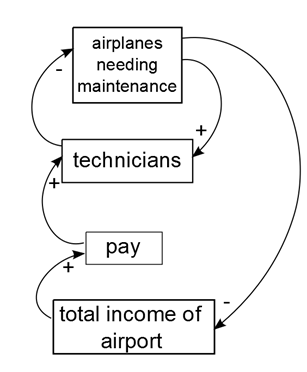
\includegraphics[width=0.45\textwidth]{pics/diaUB2} 
  \caption{System diagram}
  \label{fig:system_dia} 
 \end{figure}
  
\textbf{b)}\\
\textbf{The consumer:}\\
The customer deciding which queue to enter is best modeled as an agent. The model would address the question which queue the consumer would enter which would depend on the answers to following questions:
\begin{itemize}
  \item How many queues are free?
  \item In which queue am I going to be served the fastest?
  		\begin{itemize}
  		  \item How long are the different queues?
  		  \item How full are the carts of the others in the queue?
  		  \item How fast is the salesperson?		  
		\end{itemize}
  \item Which queue is the nearest?
\end{itemize}
The \textbf{entities} used would be: Queues , Consumers (agents), Salespersons\\
The \textbf{processes} used would be: go shopping, decide which queue to enter, pay\\\\
\textbf{The store manager:}\\
The model would address the following questions:
\begin{itemize}
  \item How many customers are in the shop at this moment?
    \item How many open queues do I need?
      \item How many customers are in average  in an hour in the shop?
        \item How many salespersons do I need 
        \item How fast are the salespersons?
        \item What is the maximum capacity of a queue?
\end{itemize}
The model would look similar to the bank office model, where queues can be added or subtracted via a slider.\\\\
\textbf{The store designer:}\\
As the store designer the task is to find the checkout area which is the most efficient one 
(= checking out 100 customers in 1 hour with the fewest employees). Using discrete event models different
kind of checkout areas are simulated (e.g. several queues, just one queue with several tellers, different
sort of queues (where there is one queue in which only customers with five or less items are allowed to check out 
or self-check out areas)). Then 100 customers will try to checkout within 1 hour. The model with the fewest tellers wins.

